\subsection{Aufbau des NAO} \label{aufbau_NAO}
%* zu softbank robotics
%* allgemeines zur größe, zu den freiheitsgraden und den Sensoren
%* Genaueres zu den Sensoren, die gemessen wurden
%* Grenzen des Naos

\begin{wrapfigure}{hr}{0.3\linewidth}
	\vspace{-1cm}
	\centering
	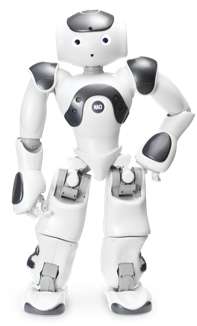
\includegraphics[width=\linewidth]{Bilder/naov6.png}
	\caption{NAO V6 \cite{nao_docu_dev_guide}}
	\label{nao_v6}
	\vspace{-2cm}
\end{wrapfigure}
NAO ist ein $574 \unit{mm}$ großer, humanoider Roboter (siehe Abb. \ref{nao_v6}) ursprünglich entwickelt von dem französischen Unternehmen Aldeberan Robotics, welche 2015 von Softbank Group aufgekauft \cite{aldebaran_to_softbank} und in Softbank Robotics umbenannt wurde. Während NAO's große Schwester Pepper mit ihren $1,20 \unit{m}$ mit einem Tablet und Rollen statt Beinen ausgestattet ist \cite{about_pepper}, gibt es NAO in verschiedenen Ausführungen, sowohl ab der Hüfte aufwärts als auch mit Beinen. Es handelt sich hier um Roboter, die unter anderem Kindern und Jugendlichen die Robotik näher bringen sollen und der Vorführung von Mensch-Roboter Interaktionen dienen. NAO bietet außerdem die Gelegenheit zweibeinige Robotersysteme zu studieren und ist bereits in psychologischen Studien verwendet worden \cite{SHAMSUDDIN20121533}. 

\begin{figure}[hb]
	\centering
	\vspace{2cm}
	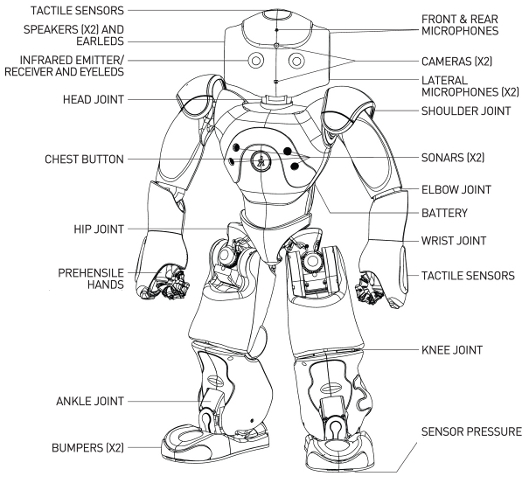
\includegraphics[width=0.75\linewidth]{Bilder/nao_h25_pres.png}
	\caption{Sensorenüberblick des NAO-H25 Version 6 \cite[in /H25]{nao_naoqi_docu}}
	\label{nao_v6_h25}
\end{figure}  

Das hier verwendete Modell ist NAO-H25 Version 6, dessen Sensoren in Abb. \ref{nao_v6_h25} zu sehen sind. Im Unterschied zu anderen Ausführungen besitzt NAO-H25 Drucksensoren an Händen und Fußsohlen. Er gehört zu den kommerziellen Robotern deren Gelenke positionsbasierenden sind \cite{balance_strategy}, hat 25 Freiheitsgrade und wiegt $5,4\unit{kg}$. Über die an der Brust angebrachten Sonar Sensoren, die Kameras oberhalb und unterhalb der Augen LEDs, die vorder- und rückseitigen Mikrofone, den Stoßfängern an den Füßen sowie den Kontaktsensoren an Händen und Kopf kann der NAO mit seiner Umwelt vielseitig interagieren. Jedes Gelenk ist mit Sensoren für die Winkelmessung, den Stromverbrauch und die Temperaturmessung ausgerüstet. In seiner Brust befindet sich außerdem ein Gyroskop. Auf die in dieser Arbeit verwendeten Messausgaben wird im Folgenden genauer eingegangen.

\subsubsection*{Druckempfindlicher Widerstand}

An den Fußssohlen des NAO befinden sich pro Fuß vier sogenannte \textit{Force Sensitive Resistors} (FSR), zu sehen in Abb. \ref{hardware_semelles}. Diese ändern ihren Widerstand sobald Druck ausgeübt wird und messen im Bereich von 0 bis $25 \unit{N}$.

Die Ausgaben der Sensoren sind im Dateiverzeichnis des NAO hinterlegt und können jederzeit ausgelesen werden. Dies geschieht hier über dasselbe Pythonprogramm, welches ebenfalls die Bewegung steuert, näheres dazu in Kap. \ref{software} und im Anhang \ref{Anhang}.
Des weiteren können der berechnete zweidimensionale Massenschwerpunkt und das Gesamtgewicht ausgegeben werden. Diese Werte sind allerdings unzuverlässig, sobald wenig oder kein Gewicht auf den Sensoren lastet. In \cite{pressure_shoe} haben Shayan et al. die eingebauten FSR mit barometrischen Drucksensoren verglichen und sind zu dem Schluss gekommen, dass die Sensoren, welche im NAO verbaut wurden, nicht sehr aussagekräftig sind. Deshalb werden hier die Ausgaben kritisch betrachtet, sowie die Balance des Roboters zusätzlich mit dem Gyroskop erfasst.
% Graph zu Gewicht des Naos (es wird weniger verzeichnet für MAP Sohlen)
\begin{figure}[tb]
	\centering
	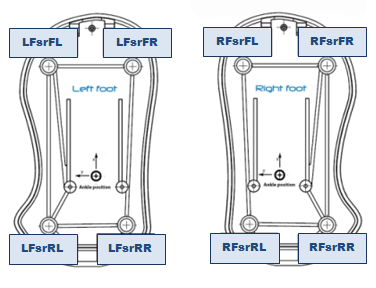
\includegraphics[width=0.6\linewidth]{Bilder/hardware_semelles.png}
	\caption{Drucksensoren und deren Bezeichnung in den Füßen von NAO \cite[ in /Technical overview/FSRs]{nao_docu_dev_guide}
	}
	\label{hardware_semelles}
\end{figure}

Eine weitere Einschränkung der Messungen ist die Kraftverteilung auf die FSRs. Denn in dem ursprünglichen unteren Teil des Schuhs liegt der obere Teil ausschließlich auf den Sensoren und auf den Verbindungszylindern für die Schrauben auf. Dies ist für die Einlegesohlen aus Silikon bzw. MAP nicht der Fall, zu sehen in den Kapiteln \ref{Schuhkonstruktion} und folgende. Dies führt dazu, dass das Gewicht nicht mehr akkurat aufgenommen wird, siehe Abb. \ref{total_weight}. Hier wird deutlich, dass sich die Messung des Gewichtes etwa um $0,5 \unit{kg}$ von den NAO Schuhsohlen abweicht. 
% Graph zu Gewicht des Naos (es wird weniger verzeichnet für MAP Sohlen)
\begin{figure}[tb]
	\centering
	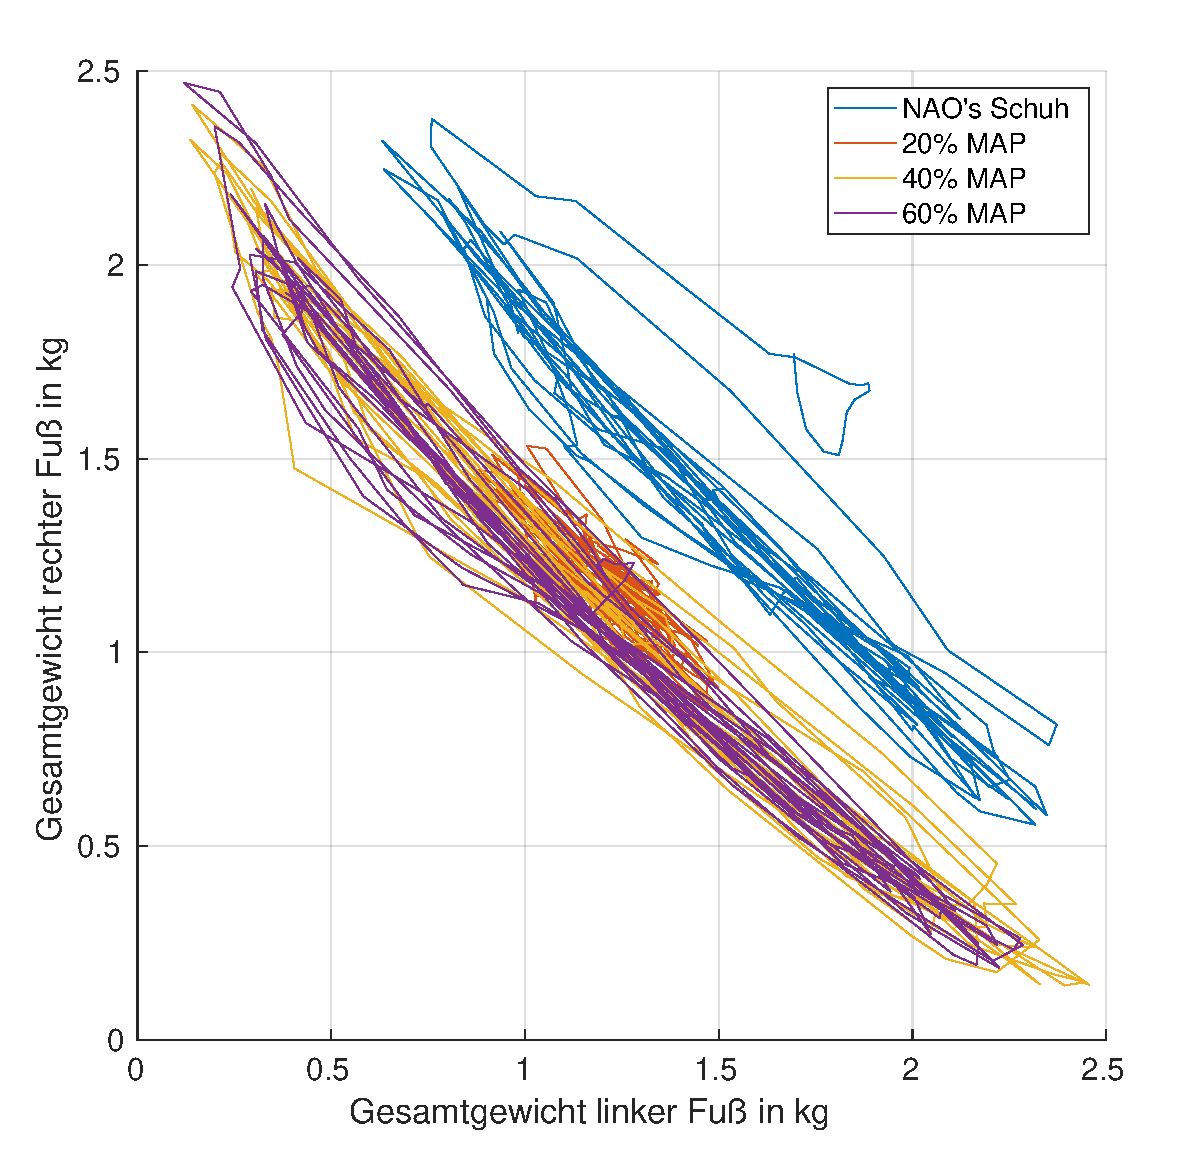
\includegraphics[width=0.8\linewidth]{Bilder/TotalWeight_Grund_20_40_60_mean.pdf}
	\caption{Berechnetes Gesamtgewicht der Messungen für die normalen Sohlen von NAO in blau und dem Silikon versetzt mit Eisenpartikeln in 20\%, 40\% und 60\% Anteilen. Das Gewicht wird in $\unit{kg}$ ausgegeben.}
	\label{total_weight}
\end{figure}

\subsubsection*{Aktoren und Sensoren der Beinen}
Neben dem für diese Arbeit uninteressanten Bumper Sensoren und den bereits beschrieben Drucksensoren hat NAO eine Ausgabe für jeden eingebauten Aktor mit den Werten:
\begin{itemize}
	\item ...\texttt{/Position/Actuator/Value} (\texttt{Pos/Act})
	\item ...\texttt{/Position/Sensor/Value} (\texttt{Pos/Sens})
	\item ...\texttt{/ElectricCurrent/Sensor/Value} (\texttt{Current})
	\item ...\texttt{/Temperature/Sensor/Value}
	\item ...\texttt{/Hardness/Actuator/Value} 
	\item ...\texttt{/Temperature/Sensor/Status} 
\end{itemize}
Hierbei unterscheiden sich die Pfade bei \glqq ...\grqq{} je nach Aktor. Die Bezeichnungen in Klammern dahinter dienen der abkürzenden Benennung für spätere Kapitel. Der Effekt der Sohlen auf die Aktoren wurde mit \texttt{AnkleRoll} und \texttt{AnklePitch} zu sehen in Abb. \ref{hardware_legjoint} aufgenommen.

\begin{figure}[b!]
	\hfill
	\begin{subfigure}[c]{\linewidth}
		\centering
		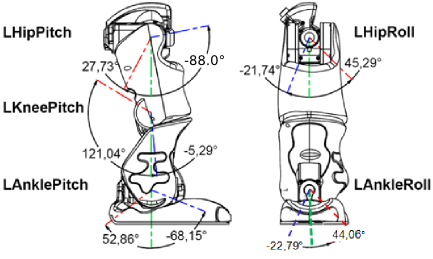
\includegraphics[width=0.7\linewidth]{Bilder/hardware_llegjoint.png}
	\end{subfigure}
	\begin{subfigure}[c]{\linewidth}
		\centering
		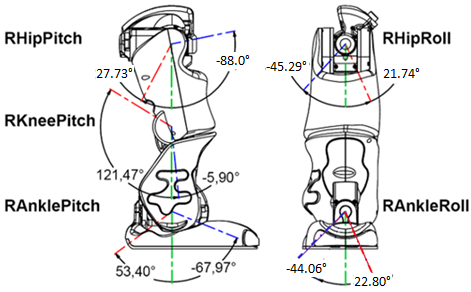
\includegraphics[width=0.7\linewidth]{Bilder/hardware_rlegjoint.png}
	\end{subfigure}
	\hfill
	\caption{Das obere Bild zeigt Vorder- und Seitenansicht der Positionen und möglichen Winkel des linken Beins. Die untere Abbildung veranschaulicht dieselben Parameter für das rechte Bein. \cite[in /kinematics-data/joints]{nao_docu_dev_guide}}
	\label{hardware_legjoint}
	%\vspace{0.1cm}
\end{figure}

Die Temperaturausgaben sowie die Starrheit der Motoren liefern keine verwertbaren Messausgaben, da sich beide während einer Messung nicht oder kaum ändern. \texttt{Pos/Act} und \texttt{Pos/Sens} geben ähnliche Werte in $\unit{rad}$ aus, da ersteres die Ausgabe des Programms vorgibt und zweiteres den tatsächlich gemessenen Wert an dem Gelenk ausgibt. Der \texttt{Current} Wert wird in Ampère gemessen und gibt an, wie viel Strom für das Erreichen der entsprechenden Aktorposition und Starrheit aufgewendet werden muss. Dies bedeutet, dass dieser Wert unter anderem eine Aussage über den Zustand des Aktors geben kann. 

Bei den Probegängen des NAO stellte sich heraus, dass er in einer Kurve nach links läuft bei einem Befehl, der ihn hätte gerade aus laufen lassen sollen. Softbank Robotics betonte, dass es nicht möglich ist, dass NAO komplett gerade läuft. Grund dafür ist zum einen, dass die Motoren nicht immer komplett identisch hergestellt sind. Zum anderen ist der Gehbefehl, welcher hier ausgeführt wird, ohne Rückkopplungsschleife für Einwirkungen der Umgebung ausgestattet. Näheres zur Software wird in Kapitel \ref{software} beschrieben.

% Jetzt kommt der Testgang und alle Graphen, die damit zusammenhängen.

% Aktoren und Sensoren in den Beinen
% Ausgabe eines Sensors und technische Details
% Wichtige Ausgaben für Stabilität
% fehlerhafter Gang

\subsubsection*{Gyroskop}
Der NAO Roboter verfügt über eine Inertialeinheit, welche sich zusammensetzt aus den 3 Achsen des Gyrometers, im einer Achsengeschwindigkeit von bis zu $500^\circ\unit{/s}$, sowie den 3 Achsen des Beschleunigungssensors, mit einer Beschleunigung bis zu $2\unit{g}$ \cite[/Technical overview/Inertial unit]{nao_docu_dev_guide}. Die Z-Achse des Gyroskops, welche die Höhenorientierung des Roboters ausgeben würde, ist allerdings noch nicht verfügbar. Außerdem wird durch diese beiden Sensoren der Winkel des Torsos bestimmt. 
\FloatBarrier

\subsection{Verwendete Software} \label{software}
\subsubsection*{Die Rahmenumgebung NAOqi}
NAOqi wird die Hauptsoftware genannt, welche auf diesem Roboter sowie auf Pepper läuft, das Betriebssystem NAOqi OS basiert auf Linux. Der NAOqi Rahmen ist eine plattformübergreifende und sprachenübergreifende Umgebung, mithilfe derer Anwendungen für den NAO erstellt werden können. Sie kann über Windows, MacOS und Linux verwendet werden und es werden die Sprachen Python und \texttt{C++} unterstützt, wobei ersteres direkt auf dem NAO kompiliert werden kann, während \texttt{C++} komplizierter benutzt wird, aber mehr Eingriffe erlaubt. \cite[/Former NAOqi Framework/Key concepts]{naoqi_dev_guide}

Außerdem gibt es eine Desktop Anwendung namens Choregraphe in der Dialoge und Verhaltensmuster erstellt werden können ohne Code schreiben zu müssen. Hierüber ist der Akkustand und aktuelle Position in Form eines virtuellen Bildes des tatsächlichen NAO einsehbar, sowie der autonome Zustand ein- und ausschaltbar. \cite[/Choregraphe Suite/What is Choregraphe]{naoqi_dev_guide}

Für die in dieser Masterarbeit benötigten Anwendungen war Python am besten geeignet. Erforderlich waren eine sich wiederholende Schrittabfolge sowie die Aufzeichnung diverser bereits im NAO verbauten Sensoren. Text verarbeitende Funktionen sind in dieser Sprache leicht zu erhalten und anzupassen. Es wurde sich für den \texttt{moveTo()} Befehl als Fortbewegungsmethode entschieden, denn dieser wird durch das Objekt \texttt{post} zu einem sogenannten \textit{non-blocking call}. Dies ermöglicht das Aufrufen von weiteren Befehlen zeitgleich zur Bewegung. Der Nachteil ist, dass der Gang dadurch unbeaufsichtigt vonstatten geht, d.h. NAO kann seine Schritte nicht seiner Umgebung anpassen. Die aufgezeichneten Daten werden in eine csv Datei übertragen und mit Matlab ausgewertet. Im Anhang ist der gesamte Programmcode \ref{Messungscode} abgebildet, welcher auf dem NAO ausgeführt wird. 

\subsubsection*{Konstruktionssoftware}	
Das CAD-Programm Inventor von Autodesk ist für 3D Konstruktionen ausgelegt und bietet einige nützliche Simulationserweiterungen, welche unter anderem einen Shape Generator enthält \cite{inventor}. Dieser kann Flächen minimieren während die Stabilität erhalten bleibt, sodass ein minimaler Anteil an Material verwendet wird \cite{shape_generator}. 

Für die Herstellung der Prototypen und Gussformen wurde das FDM (fused deposition modeling) 3D Druckverfahren mit PLA oder PETG Filamenten von filamentworld \cite{filament} verwendet und für die Vorbereitung auf den Druck der Slicer Cura von Ultimaker \cite{cura}.

\subsubsection*{Datenauswertung mit Matlab}
Für die Auswertung wurden neben der gewöhnlichen \texttt{plot} Funktion von Matlab \cite{matlab} auch die \textit{Statistics and Maschine Learning} Toolbox mit deskriptiver Statistik und Visualisierung verwendet \cite{toolbox}. 
Eine Messreihe ergibt sich aus 40 Messungswiederholungen, in denen NAO etwa einen Meter zurücklegt. Jede Auswertung enthält das arithmetische Mittel eines Sensors von allen Messungen der Messreihe. Diese Mittel wurden mit dem Befehl \texttt{mean()} berechnet und mit Werten aus weiteren Messreihen, mit anderem Schuh oder anderen Untergrundvoraussetzungen aber gleicher Schrittlänge und Sensorenmessung verglichen. Dieser Vergleich wurde mit den Funktionen \texttt{hist} und \texttt{scatterhist} der genannten Toolbox angestellt. Ersteres erstellt ein Histogramm und ist damit optimal für eine Häufigkeitsverteilung. Zweiteres erstellt einen aus zwei Vektoren resultierenden Scatterplot sowie zwei Histogramme, welche die Häufigkeitsverteilung der jeweiligen Vektoren darstellen. Dies ermöglicht eine umfangreiche Verteilungsanalyse für Sensorausgaben, die sich aus zwei Achsen zusammensetzen, wie z.B. der 2 dimensionalen Gyroskop Ausgabe.

Das arithmetische Mittel berechnet Matlab durch \cite[S.50]{statistik_Ludwig}
\begin{equation}
	\bar{x} = \frac{1}{n} (x_1 + x_2 + \dots + x_n) = \frac{1}{n}\sum_{i=1}^{n}x_i
\end{equation}
und wurde auf eine Messreihe angewendet. Die Darstellung der Verteilungen per Histogramm wurde ergänzt durch ein gleitendes Histogramm, errechnet durch den Kern-Dichteschätzer \cite[S.93]{statistik_Ludwig}
\begin{align}
	\hat{f}(x)=\frac{1}{nh} \sum_{i=1}^{n}K\left(\frac{x - x_i}{h}\right),\, x \in \mathds{R}
\end{align}
mit dem Gauss-Kern \cite[S.93]{statistik_Ludwig}, 
\begin{align}
	K(u) = \frac{1}{\sqrt{2\pi}} \exp\left(-\frac{1}{2}u^2\right),\, u \in \mathds{R}
\end{align}
welcher in Matlab mit \texttt{'Kernel'} und dann standardmäßig mit \texttt{'normal'} in der \texttt{fitdist()} Funktion aufgerufen wird \cite{kernel-distribution} \cite{fitdist}. Das Scatterhistogramm ermöglicht dieselbe Verwendung dieser Distribution. 


\FloatBarrier
\subsection{Magneto-aktive Polymere}\label{kap_MAP}
%	 woher kommt der begriff, was ist es
%	 woher bestand die bisherige Forschung, warum ist es interessant
\subsubsection*{Begriffserklärung und Eigenschaften}
Der Begriff Magneto-Aktive Polymere (MAP) gehört zur Gruppe der intelligenten, auf magnetische Felder ansprechende Materialien, welche typischerweise Kombinationen aus einer weichen Polymermatrix und darin eingebetteten, magnetischen Partikeln sind. Diese Partikel werden während dem Vernetzungsprozess des Polymers in dieses eingebettet. 

Die wesentlichen Verhaltensweisen, die MAP in der heutigen Zeit attraktiv für seine Verwendung macht, wurde bereits in den 80ger Jahren von Rigbi und Jilken \cite{Rigbi1} sowie Rigbi und Mark \cite{Rigbi2} beschrieben. Ein Jahrzehnt später wurde eine genauere Analyse zum ersten Mal von Ginder und Jolly et al. \cite{ginder} veröffentlicht. 
Diese aus mehreren Komponenten bestehenden Materialien stechen durch zwei Schlüsseleigenschaften heraus. 
Zum einen das magnetostriktive Verhalten, bei dem es sich um das Phänomen der Verformung eines Materials handelt, welches durch ein Magnetfeld hervorgerufen wird \cite{Martin_2006}.
Zum anderen die veränderbaren Materialeigenschaften wie Elastizität und Dämpfungsfaktor, welche hauptsächlich mit der Mikrostruktur des Grundlagenmaterials zusammenhängen. \cite{Varga1} \cite{Varga2}

Außerdem ist entscheidend, wie die magnetischen Partikel in das Polymer eingebettet werden. Je nachdem ob während des Vernetzungsprozesses ein Magnetfeld wirkt, können sich die Partikel kettenförmig ausrichten und dadurch dem MAP eine anisotropisches Verhalten zuführen. Isotropisches MAP hingegen enthält keine gerichteten Partikel. Diese verschiedenen Ausrichtungsarten und Herstellungsarten können sowohl die Steifigkeit verändern, als auch bestimmen, ob das MAP in einem Magnetfeld ausgedehnt oder zusammengedrückt wird. 

Weiche, mit einem Feld manipulierbare, Polymere haben diverse Anwendungsbereiche in akademischen und industriellen Bereichen. Angefangen von anpassungsfähiger Vibrationsabsorption in der Luftfahrt und Automobilindustrie durch das Einsetzen durch Scherung \cite{Ginder_Schlotter_Nichols} \cite{Deng_Gong}, Windung \cite{Hoang_Zhang_Li_Du} und Kompression bzw. Elongation \cite{Kallio_2007} und Vibrationsisolatoren \cite{Ginder_2000} sowie Sensoren \cite{Ginder_2000} \cite{Martin_2006}, Ventile und Aktoren \cite{Boese_2012} \cite{Keip_2014} und anpassungsfähige, sandwichartige Strukturen \cite{Zhou_2005} \cite{Zhou_2006} \cite{Wei_2008} bis hin zur Anwendung in der Bionik wie zum Beispiel durch Mikro- und Nanoroboter und Schwimmroboter \cite{Qiu_2015} \cite{Xu_2015} \cite{Lum_2016} \cite{Hu_2018}, Schlauchradpumpen \cite{Fuhrer_2013} und Erschütterungsdämpfer \cite{Li_2013}.

Des Weiteren wird die Verhärtung bei Anlegen eines Magnetfeldes für Greifer genutzt \cite{Qi_2020}, ebenso wird der 3D Druck von magneto-aktiven Polymeren \cite{Sindersberger_2018} bereits erforscht.

\subsection{Magnetostiction}

Der Begriff Stiction ist in erster Linie eine englische Wortneuschöpfung aus dem Wort \textit{friction}, also Reibungskraft und \textit{sticking}, also kleben. Ersteres wird unterschieden in Haftreibung, welche den Schwellenwert einer äußeren Kraft darstellt, der überwunden werden muss um ein Objekt in Bewegung zu versetzen, sowie in Gleitreibung, welche den Widerstand, der entgegen der Bewegungsrichtung wirkt, beschreibt. Stiction entsteht wenn die Haftreibung die Gleitreibung übersteigt. Dies sorgt für einen plötzlichen Stillstand, bis dann die auf das Objekt wirkende Kraft ausreicht, um eine erneute Bewegung zu erlauben. Dies kann zu ruckartigen Bewegungen führen und ist deshalb in vielen Fällen eine unerwünschte Eigenschaft \cite{Ruel2014STICTIONT}. Es gilt dies nicht zu verwechseln mit Adhäsion, welche entsteht, wenn z.B. Silikon auf dem Boden flach aufliegt und sich an den Boden auf die Art anpasst, dass bei dem Versuch, es zu schieben, sich an den Boden anklebt. Wenn die Adhäsion fehlt, aber die Reibung noch kontrollierbar ist, dann handelt es sich um Stiction. \cite{Monkman_2019}


	
%%% Local Variables:
%%% mode: latex
%%% TeX-master: "main"
%%% End: